\chapter{Methodology}\label{ch:methodology}

This chapter combines the prediction problem and the PHGST-DM methodology into one account, following the structure of the final report. The system definition and targets are introduced first; subsequent sections explain how observations are transformed into supervision, how structural and temporal information is encoded, and how the model produces and selects bottleneck reports. All reported methods are those used in the PHGST-DM study; unrelated sensing and detection components are outside the scope of this chapter.

\section{Overall Framework and Problem Formulation}\label{overall-framework-and-problem-formulation}

\subsection{Overall Framework of PHGST-DM}\label{overall-framework-of-phgst-dm}

PHGST-DM integrates four connected elements: a traceable factory-model data source, process-informed event construction, a heterogeneous graph representation, and a delay-aware multi-task predictor. The factory model records resource states and job progress; second-resolution observations are aggregated into aligned windows. Resource-specific operating evidence and persistence rules define supervision, while production and logistics relations define the graph. Grouped features and attention mechanisms, including temporal-pattern conditioning, provide the representations used to produce bottleneck-event and auxiliary outputs.

As illustrated in Figure~\ref{fig:overview},
the framework transforms factory observations
into aligned temporal windows and process-informed
supervision, constructs a heterogeneous resource
graph, and applies delay-aware spatiotemporal
modelling to generate joint bottleneck predictions.

\begin{figure}[!htbp]
\centering
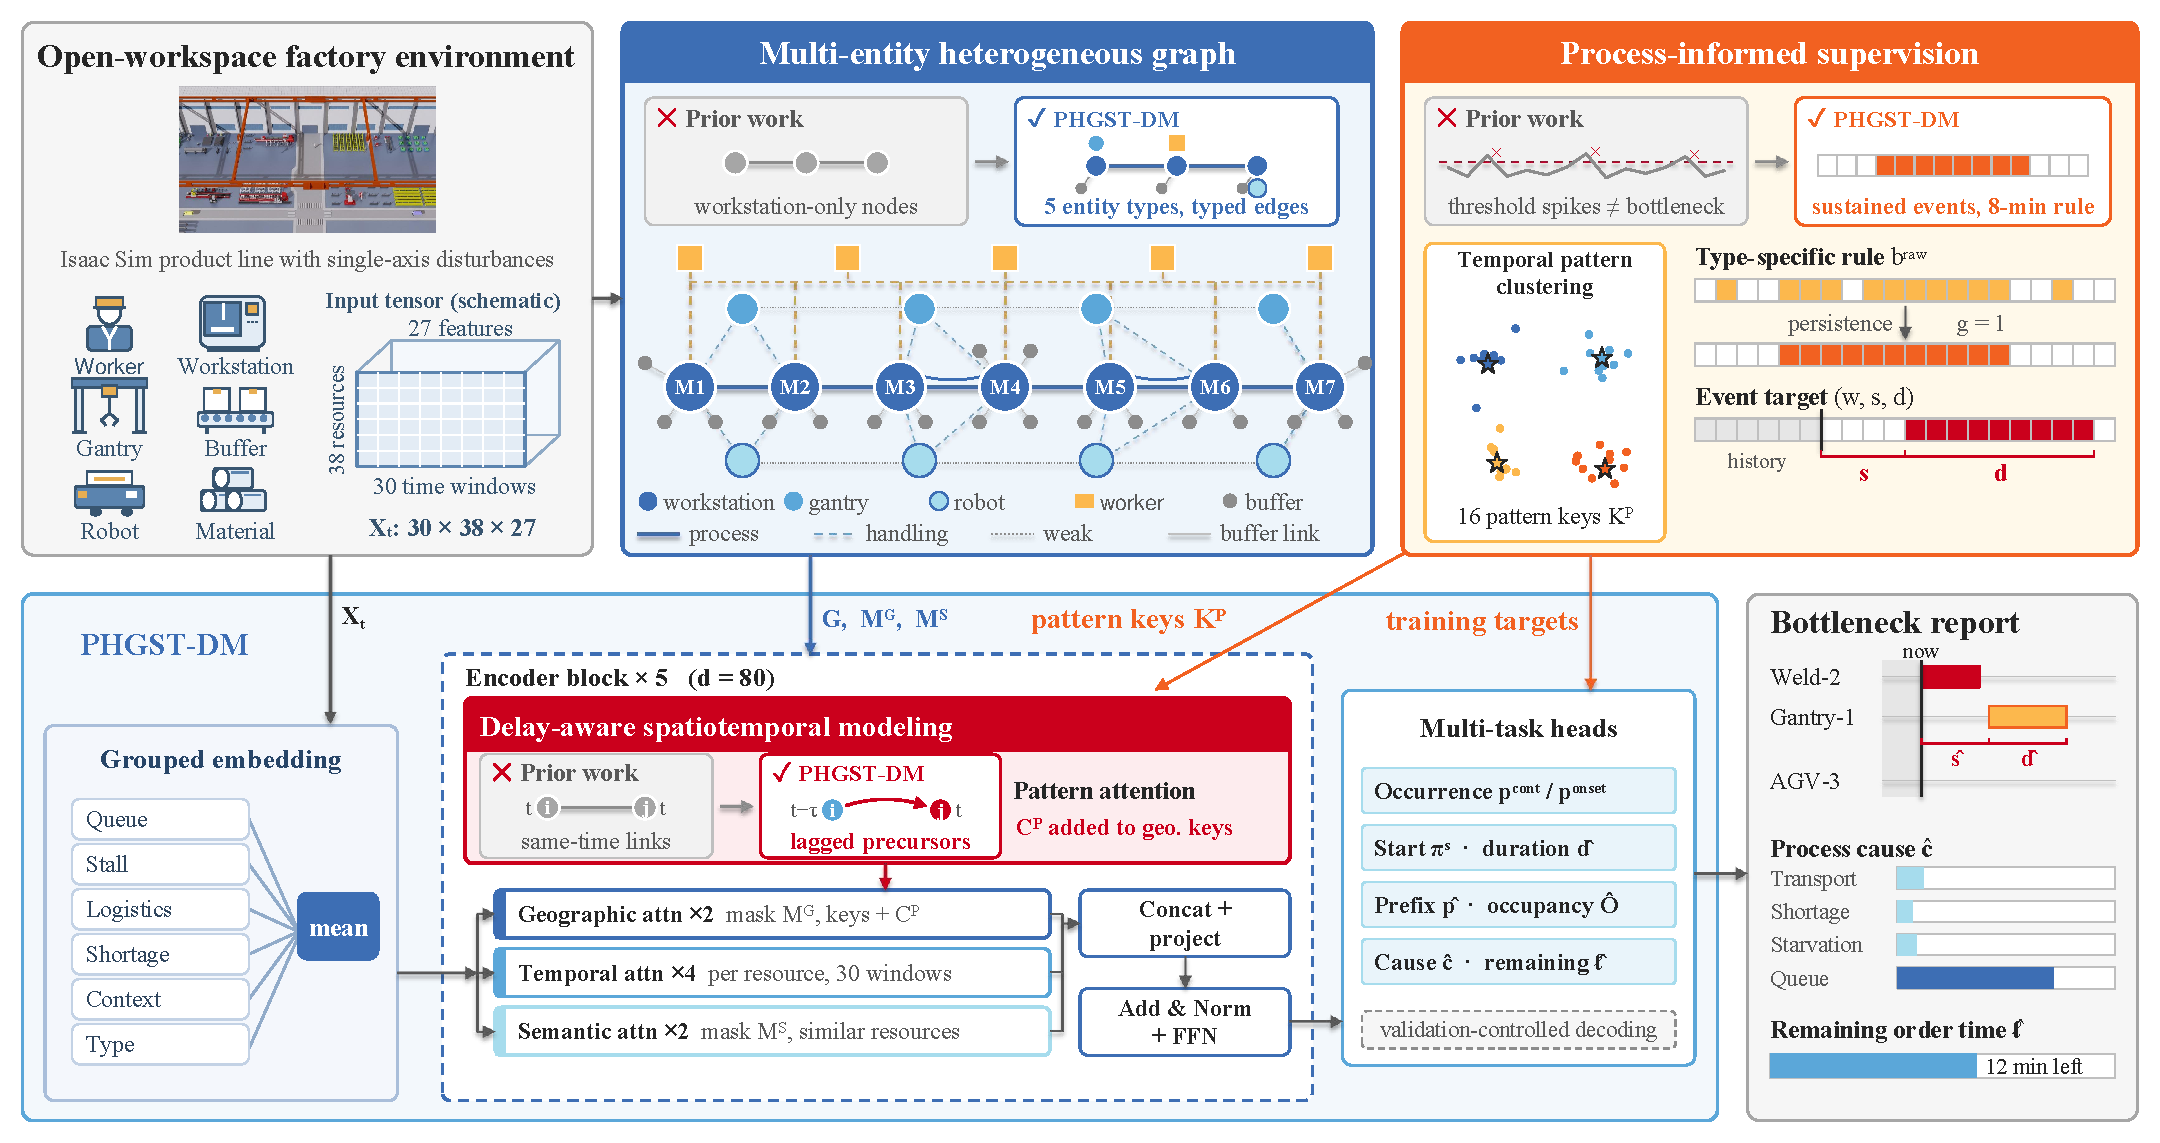
\includegraphics[width=\linewidth,height=0.58\textheight,keepaspectratio]{figures/fig_method_final.pdf}
\caption{Overall PHGST-DM framework: multi-entity observations, process-informed supervision, graph-based delay-aware encoding, and a structured bottleneck report.}
\label{fig:overview}
\end{figure}
\FloatBarrier

The model operates on production histories generated by a controlled factory process. Its role is to predict future constraints rather than to replace the admission, allocation, or task-planning controllers running the factory. Evaluation of the resulting forecasts is reported separately in Chapter~\ref{ch:experiments}.

Algorithm~\ref{alg:phgst-train} formalizes the complete training and model-selection pipeline. Algorithms~\ref{alg:targets}--\ref{alg:phgst-predict} detail its supervision, fixed context, and prediction steps. The retained event model and report threshold are specific to each onset-limit setting; the curriculum transfers a checkpoint between settings, while remaining-time specialization preserves each selected event operating point.

\begin{algorithm}[p]
\singlespacing
\footnotesize
\SetAlFnt{\footnotesize}
\SetAlCapFnt{\small}
\SetAlCapNameFnt{\small\bfseries}
\SetInd{0.5em}{0.8em}
\caption{End-to-end PHGST-DM training, selection, and held-out evaluation.}
\label{alg:phgst-train}
\KwIn{raw episodes $\mathcal{E}$; factory relations $G$; onset limits $\mathcal{H}=\{5,10,15\}$; candidate thresholds $\mathcal{T}$}
\KwOut{frozen event model $\theta^{\star}$, remaining-time head $\psi^{\star}$, threshold $\tau^{\star}$, held-out reports}
\BlankLine
\textbf{Phase 1: leakage-controlled data and fixed structural context}\;
split $\mathcal{E}$ by episode into $\mathcal{E}_{\mathrm{tr}},\mathcal{E}_{\mathrm{val}},\mathcal{E}_{\mathrm{te}}$\;
construct samples with history-only inputs using Algorithm~\ref{alg:targets}, independently within each episode\;
fit all feature/target scalers on $\mathcal{E}_{\mathrm{tr}}$; reuse them unchanged for $\mathcal{E}_{\mathrm{val}}$ and $\mathcal{E}_{\mathrm{te}}$\;
obtain $(A,M^{G},M^{S},E_{\mathrm{lap}})$ from Algorithm~\ref{alg:graph-masks} and $K^{P}$ from Algorithm~\ref{alg:pattern-bank}\;
freeze every data-derived structural quantity before neural-parameter optimization \tcp*{masks and prototypes stay fixed}
\BlankLine
\textbf{Phase 2: shared-representation learning (training stage 1)}\;
initialize $\theta$ from the documented prefix-supervised checkpoint\;
\ForEach{$H_{\mathrm{start}}\in\mathcal{H}$ in curriculum order}{
warm-start the current onset limit from the preceding retained checkpoint when available\;
  \For{epoch $=1,\ldots,E_1$ ($E_1=50$) until patience is exhausted}{
    \ForEach{oversampled training minibatch $B$}{
$(\widehat{Y}^{\mathrm{evt}},\hat O,\hat c,\hat\ell)\leftarrow\mathrm{PHGSTDMForward}_{\theta}(B,A,M^{G},M^{S},K^{P})$\;
evaluate the event, occupancy, cause, reconstruction, contrastive, and remaining-time losses, then update $\theta$\;
    }
decode $\mathcal{E}_{\mathrm{val}}$ with Algorithm~\ref{alg:phgst-predict} for every $\tau\in\mathcal{T}$\;
retain checkpoints and thresholds by the validation rules in Section~\ref{sec:experimental-settings}, including the validation-only fallback\;
  }
}
freeze the selected stage-1 parameters and threshold as $(\theta^{\star},\tau^{\star})$ \tcp*{event reports locked hereafter}
\BlankLine
\textbf{Phase 3: remaining-time specialization (training stage 2)}\;
freeze the encoder and all event, occupancy, and cause heads\;
initialize the rate-augmented remaining-time head $\psi$ from $\theta^{\star}$\;
\For{epoch $=1,\ldots,E_2$ ($E_2=20$) until validation loss stops improving}{
update only $\psi$ using progress-weighted remaining-time loss\;
}
freeze $\psi^{\star}$; do not retune $\tau^{\star}$\;
\BlankLine
\textbf{Phase 4: held-out evaluation after all choices are frozen}\;
run Algorithm~\ref{alg:phgst-predict} on $\mathcal{E}_{\mathrm{te}}$ using $(\theta^{\star},\psi^{\star},\tau^{\star})$\;
\Return frozen models, threshold, and held-out reports \tcp*{test episodes never re-enter selection}
\end{algorithm}
\FloatBarrier

\subsection{Production System and Resource Relations}\label{production-system-and-resource-relations}

The evaluated production system processes an order of ten workpieces through cutting, grooving, spot welding, root welding, surface welding, and finishing. The operation also involves worker service, intermediate storage, gantry handling, and AGV transportation. In this report, a \textbf{workstation} is a processing or assembly unit, including automated equipment and manually operated workbenches.

Let \(\mathcal{R}\) be the set of all resources, partitioned into workstations, gantries, transport robots, workers, and buffers:

\[
\mathcal{R}=\mathcal{R}^{m}\cup\mathcal{R}^{g}\cup\mathcal{R}^{a}\cup\mathcal{R}^{h}\cup\mathcal{R}^{b}.
\]

The evaluated graph contains 38 nodes. Event supervision is restricted to workstations, gantries, and AGVs:

\[
\mathcal{S}=\mathcal{R}^{m}\cup\mathcal{R}^{g}\cup\mathcal{R}^{a}.
\]

\begin{table}[!htbp]
\centering
\caption{Heterogeneous graph entities and their supervision roles.}
\label{tab:resources}
\small
\begin{tabularx}{\linewidth}{@{}l c X@{}}
\toprule
Resource type & Nodes & Role in the representation \\
\midrule
Workstations & 7 & Processing and assembly; event-supervised \\
Gantries & 4 & Handling services; event-supervised \\
Transport robots (AGVs) & 4 & Transportation; event-supervised \\
Workers & 5 & Labour availability and service context \\
Buffers & 18 & Storage and WIP context \\
\midrule
\textbf{Total} & \textbf{38} & \textbf{15 event-supervised resources} \\
\bottomrule
\end{tabularx}
\end{table}
\FloatBarrier

Worker and buffer nodes provide predictive context but are not assigned separate event targets. Materials are not added as independent graph nodes: their effects enter through shortage, inbound-waiting, and buffer-related features associated with existing resources.

The factory relations are represented by a \textbf{weighted undirected graph}:

\[
G=(\mathcal{R},E,A),\qquad E=E^{p}\cup E^{f}\cup E^{b}\cup E^{l}\cup E^{w},
\]

where \(A\) is the symmetric weighted adjacency matrix. The five edge groups represent process-chain links, parallel workstations in the same equipment family, buffer--workstation associations, handling--processing links, and same-type handling links, respectively. Edges encode structural relations that permit information exchange; they should not be interpreted as experimentally established physical causal pathways.

\subsection{Windowed State and Joint Prediction Targets}\label{windowed-state-and-joint-prediction-targets}

Operational records are aggregated into non-overlapping windows of \(\Delta=60\,\mathrm{s}\). Each resource has a 27-dimensional state vector \(x_{t,n}\in\mathbb{R}^{27}\), consisting of 21 operational variables, five resource-type indicators, and one labour-saturation variable. The operational features are divided into six semantic groups:

\begin{table}[!htbp]
\centering
\caption{Semantic feature groups in the final model.}
\label{tab:features}
\small
\begin{tabularx}{\linewidth}{@{}l c X@{}}
\toprule
Group & Dimension & Representative information \\
\midrule
Queue & 4 & Queue length, waiting, occupancy, growth \\
Stall & 6 & Blocked/starved time, stop, availability, coupling \\
Logistics & 4 & Departure variation, route/inbound delay, buffer \\
Shortage & 1 & Material-shortage propagation \\
Context & 7 & Activity, duration, time gap, operating variation, turning state, labour \\
Type & 5 & Workstation, gantry, worker, robot, buffer \\
\midrule
\textbf{Total} & \textbf{27} & \\
\bottomrule
\end{tabularx}
\end{table}
\FloatBarrier

Labour saturation is derived from worker states and provided to workstations. The exported \emph{offline bottleneck score} is \textbf{excluded} from predictive inputs, preventing the model from simply reproducing its own supervision score. With forecast origin \(t\), historical length \(T_{\mathrm{in}}=30\), and \(N=38\) nodes, the input is

\[
X_t=\bigl[x_{\tau,n}\bigr]_{\substack{\tau=t-T_{\mathrm{in}},\ldots,t-1\\n=1,\ldots,N}}
\in\mathbb{R}^{T_{\mathrm{in}}\times N\times27}
=\mathbb{R}^{30\times38\times27}.
\]

The future occupancy-label grid contains \(H_{\mathrm{label}}=30\) one-minute windows. A newly starting event is eligible for a report only if its onset lies within a separate \textbf{onset limit} \(H_{\mathrm{start}}\in\{5,10,15\}\) minutes. The onset limit restricts the admissible \emph{start} of a new event; it does not shorten the fixed 30-minute future label grid.

For supervised resource \(n\), the event target is

\[
y^{\mathrm{evt}}_{t,n}=(w_{t,n},s_{t,n},d_{t,n}),
\]

where \(w_{t,n}\) is event occurrence, \(s_{t,n}\) is onset offset, and \(d_{t,n}\) is future event length, all temporal quantities being expressed in one-minute windows. The model also estimates a graph-level process-cause class \(c\) and line-level remaining-order time \(\ell\).

The corresponding predictive mapping is

\[
f_{\theta}:(X_t,G)\longmapsto
\left(\{\hat w_{t,n},\hat s_{t,n},\hat d_{t,n}\}_{n\in\mathcal{S}},\;\hat c_t,\;\hat\ell_t\right),
\]

with parameters \(\theta\). Although the report is generated at \(t\), individual target construction and inference use different temporal information; Section~\ref{data-preparation-and-process-informed-supervision} makes that distinction explicit.

\section{Data Preparation and Process-informed Supervision}\label{data-preparation-and-process-informed-supervision}

\subsection{Open-workspace Factory Model and Data Collection}\label{open-workspace-factory-model-and-data-collection}

The NVIDIA Isaac Sim factory model records resource transitions, processing and job traces, buffer changes, transport tasks, and inventory at logical-second resolution. Streams are synchronized by episode identifier and logical time. In the evaluated setup, a completed episode contains ten finished workpieces. Episodes affected by the documented simulator deadlock defect are discarded as invalid records, rather than being used as normal production trajectories.

The data-generation environment supports configurable changes to \textbf{workstation}, \textbf{worker}, \textbf{logistics}, and \textbf{material} operating conditions. Each variation dimension can affect episode-wide capacity, sampled service behaviour, or temporary runtime events; the evaluated \texttt{dense\_i1} collection activates a single variation dimension at intensity level 1, alongside nominal episodes. Full disturbance settings, episode counts, and train/validation/test composition belong to Chapter~\ref{ch:experiments}. Critically, the category used to generate an operating variation is \emph{not} copied directly into the process-cause label: supervision is derived from observed states following the variation.

\begin{figure}[!htbp]
\centering
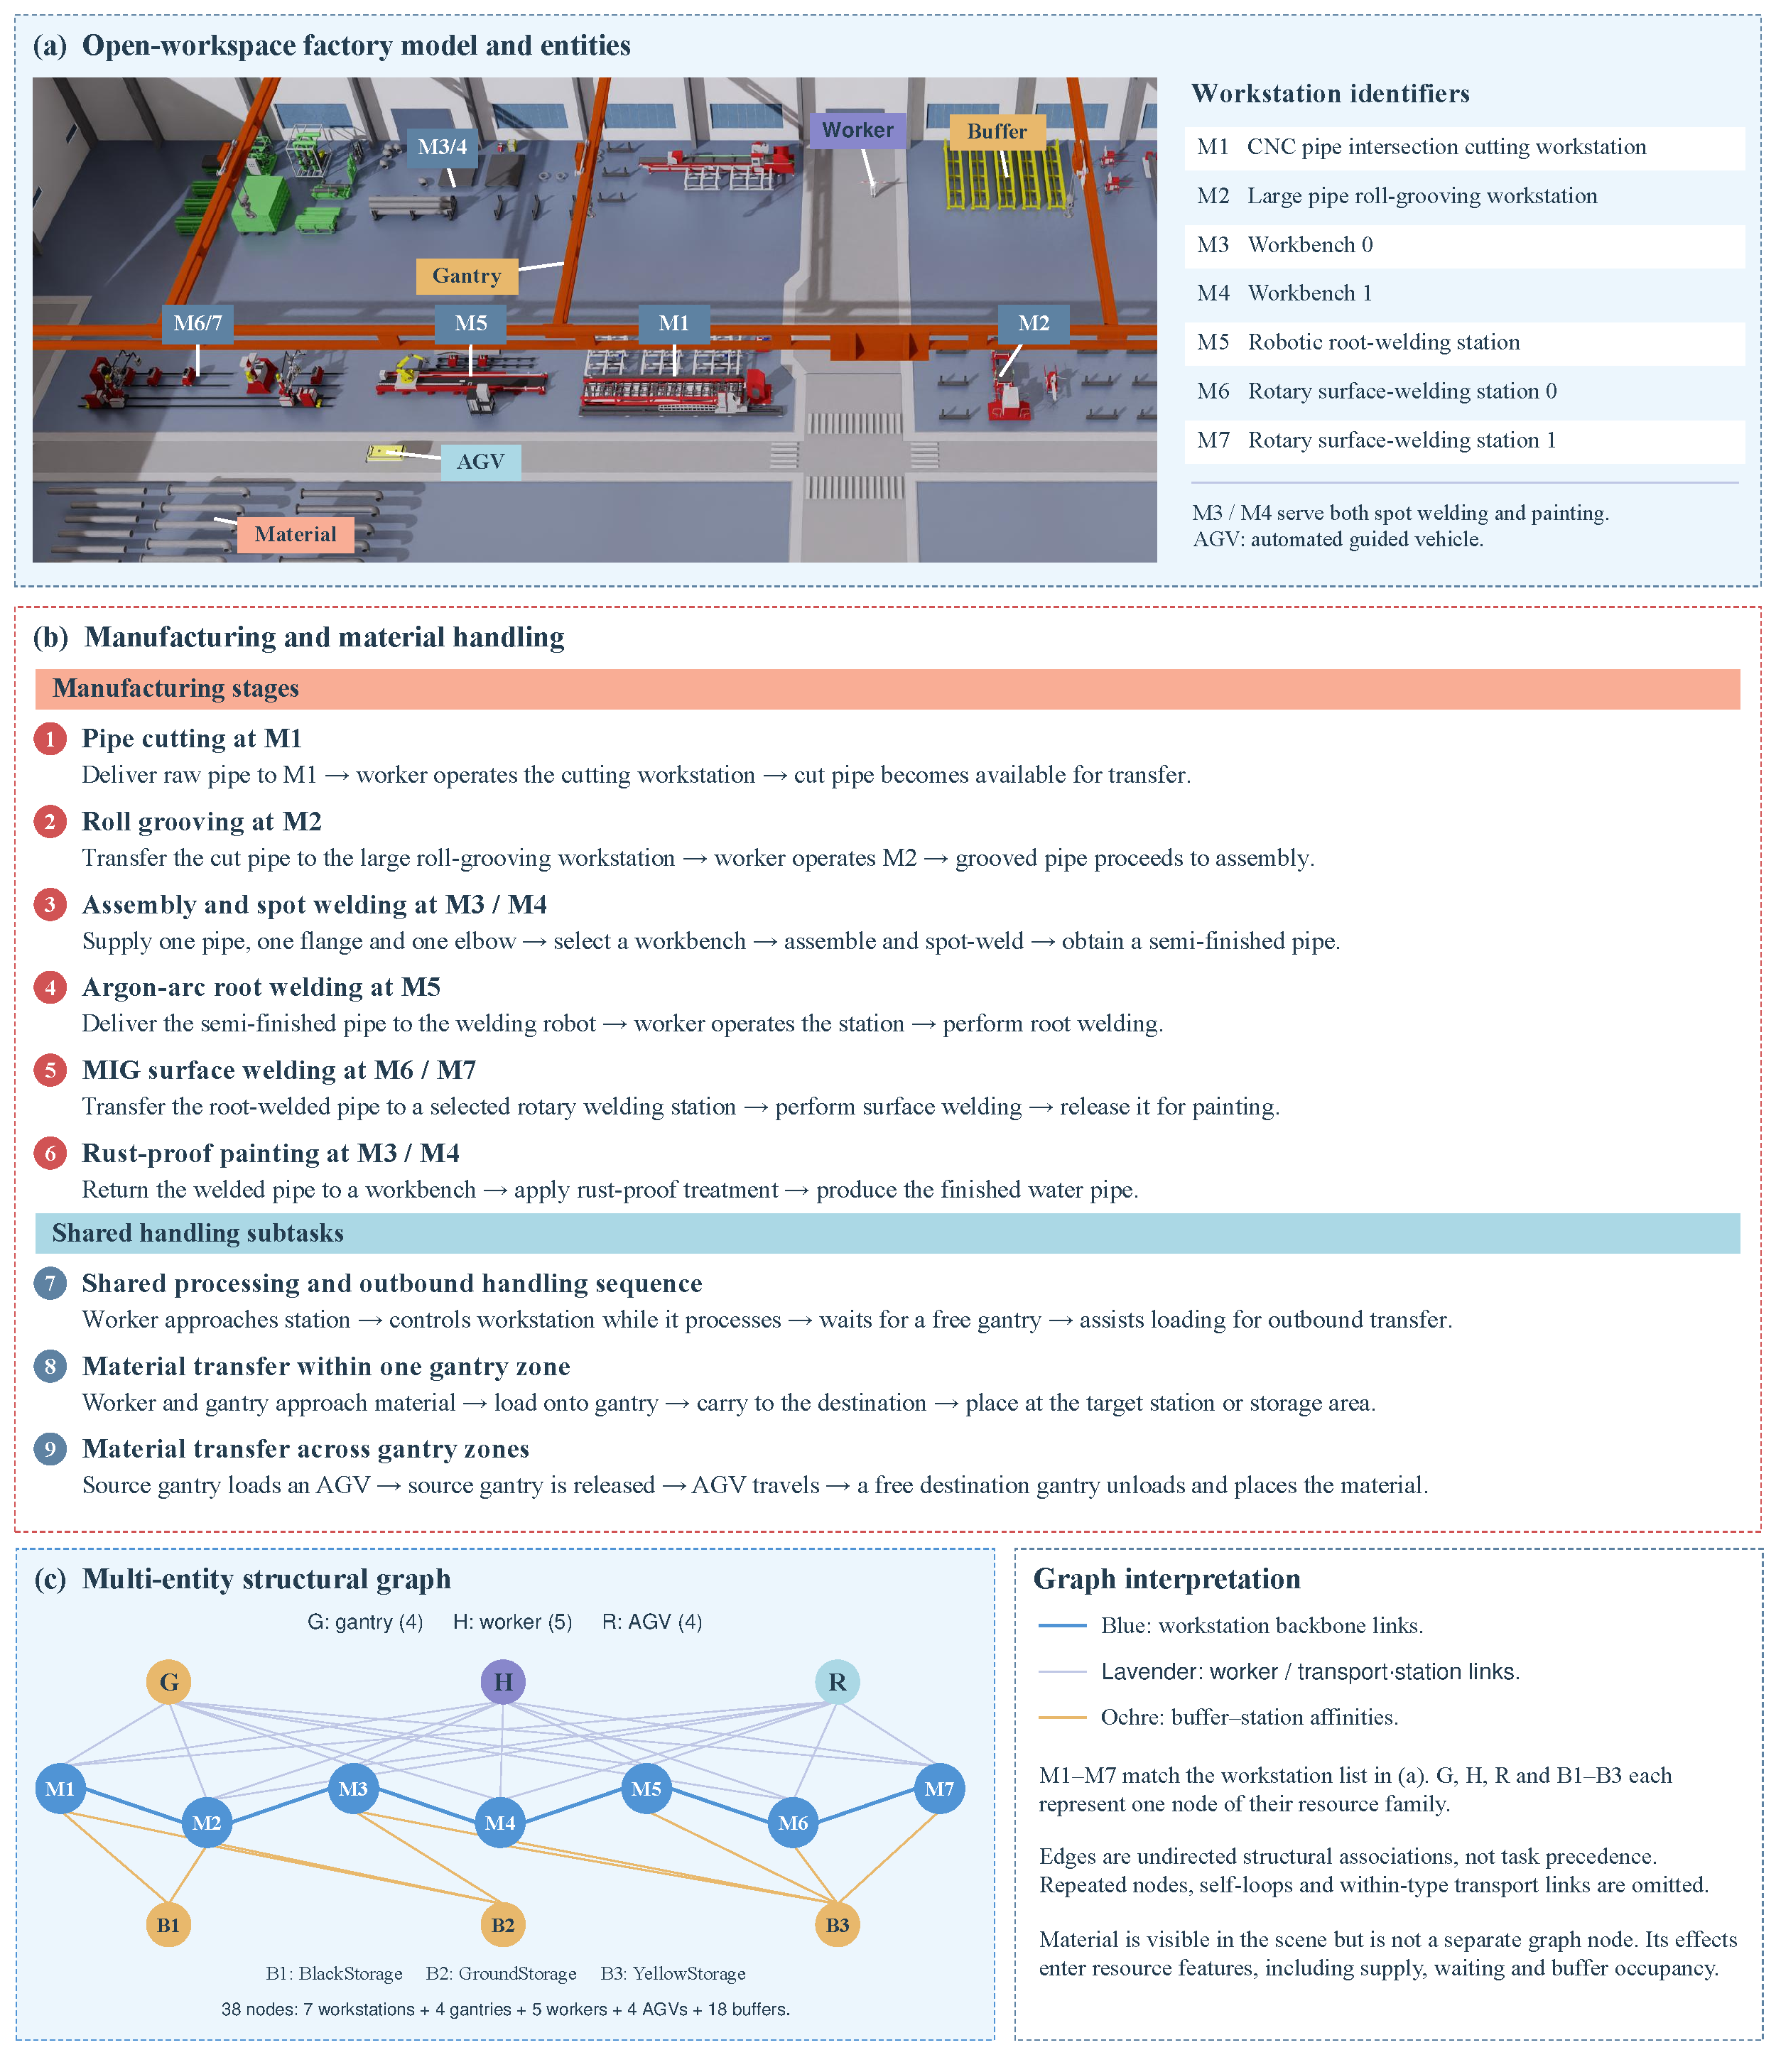
\includegraphics[width=\linewidth,height=0.70\textheight,keepaspectratio]{figures/fig_experiment.pdf}
\caption{Isaac Sim production environment, manufacturing and handling stages, and the heterogeneous graph of 38 resources.}
\label{fig:factory}
\end{figure}
\FloatBarrier

\subsection{Multi-entity Aggregation and Regime Context}\label{multi-entity-aggregation-and-regime-context}

Second-resolution logs are transformed into resource-by-window observations. Processing, blockage, starvation, and stoppage durations are accumulated according to their overlap with a 60-second window; activity and unavailability ratios are normalized by the window length. Queue statistics count waiting jobs and summarize waiting time. Buffer occupancy is averaged within the window, its previous value is carried forward when no update is recorded, and growth is computed from window-end minus window-start counts. Production and transport relations are used to derive coupling information, route delay, inbound waiting, and shortage propagation.

A fixed resource ordering aligns the heterogeneous channels across all episodes. Missing numeric entries are filled with zero, type indicators are appended, and labour saturation is recomputed from worker activity. Histories are generated using a one-window stride without crossing episode boundaries. Standardization is fitted \textbf{only on training histories} and reused unchanged for validation and testing.

The run-stratified episode split contains 140 training, 28 validation, and 36 test episodes, giving 20,826, 4,331, and 5,354 forecast windows, respectively (Table~\ref{tab:exp-dataset}). Splitting by complete episode precedes fitting scalers, semantic masks, and temporal prototypes; overlapping histories never cross episode boundaries. The disturbance protocol is specified in Table~\ref{tab:disturbance-design}, while baseline definitions and evaluation metrics are given in Tables~\ref{tab:exp-baselines} and~\ref{tab:exp-metrics}. These settings define the evaluation procedure without duplicating the results in Chapter~\ref{ch:experiments}.

The method distinguishes three related but non-equivalent objects. \textbf{Process-cause labels} represent observed operating symptoms accompanying bottleneck evidence. \textbf{Deterministic regime identifiers} are generated by cause-aligned rules to provide representation and contrastive-learning context. \textbf{Temporal-pattern prototypes} are clustered from training activity histories and subsequently used for attention conditioning (Section~\ref{recurrent-pattern-guided-delay-aware-spatiotemporal-modelling}). Neither regime IDs nor temporal clusters should be mistaken for independently verified bottleneck truth.

\subsection{Construction of Sustained Bottleneck Events}\label{construction-of-sustained-bottleneck-events}

Raw resource evidence must distinguish an operationally meaningful constraint from ordinary resource activity or a brief fluctuation. For resource type \(\rho(n)\), the rule \(\Phi_{\rho(n)}\) maps resource state and observed process information to a binary hot indicator:

\[
b^{\mathrm{raw}}_{t,n}=\Phi_{\rho(n)}(x_{t,n},X_t)\in\{0,1\}.
\]

Workstation evidence combines queue conditions, blockage/starvation, availability, coupling to upstream or downstream resources, inbound waiting, route delay, shortage propagation, and labour conditions. Gantry and AGV rules place greater emphasis on handling-related waiting and unavailability. The threshold conditions are applied to \textbf{physical-scale} features before standardization, rather than arbitrary normalized values. Table~\ref{tab:raw-hot} gives representative rules rather than an exhaustive list of workstation conditions.

\begin{table}[!htbp]
\centering
\caption{Selected examples of resource-specific raw-hot evidence (non-exhaustive). Here $q$ is queue length, $B$ blocked seconds, $S$ starved seconds, $I$ inbound-wait seconds, $R$ route-delay seconds, and $U$ unavailable fraction.}
\label{tab:raw-hot}
\small
\begin{tabularx}{\linewidth}{@{}p{2.35cm} X@{}}
\toprule
Resource & Representative raw-hot conditions (logical OR) \\
\midrule
Workstation & $q\geq2$ and $B+S>0$; or $B\geq24$ s and $q\geq1$; other stall/coupling/shortage/labour conditions also apply \\
Gantry & $B+S\geq18$ s and ($I\geq20$ s or $R\geq20$ s); or $U\geq0.5$ \\
AGV & $B+S\geq18$ s and $I\geq20$ s; or $U\geq0.5$ \\
\bottomrule
\end{tabularx}
\end{table}
\FloatBarrier

To remove transient positives, a short-run filter \(\mathcal{D}_m\) first drops raw positive runs shorter than \(m=8\) one-minute windows. A subsequent internal-gap operator \(\mathcal{F}_g\) fills gaps of at most \(g=1\) window between retained regions. The offline sustained occupancy sequence is therefore

\[
o_{:,n}=\mathcal{F}_{1}\!\left(\mathcal{D}_{8}\!\left(b^{\mathrm{raw}}_{:,n}\right)\right).
\]

The ordering matters: \textbf{short-run removal precedes internal gap filling}. This occupancy grid is an \emph{offline target} obtained from the full episode and may retrospectively use later observations to decide whether an earlier period belongs to a sustained event. At forecast origin \(t\), the predictor must instead use the \textbf{history-only} state \(h_{t-1,n}\) computed exclusively from windows strictly before \(t\), including prefix-based persistence and gap checks. In general, \(h_{t-1,n}\) need not equal the retrospective \(o_{t-1,n}\).

An event is \textbf{ongoing} if the history-only state is active and the future run starts at offset zero; its target duration is the remaining future length. A newly appearing run with positive onset offset is \textbf{upcoming} if its onset lies within \(H_{\mathrm{start}}\) and it satisfies the minimum-duration rule. Where multiple eligible runs are available for one resource, the \textbf{longest} qualifying run is selected, rather than always the earliest. This defines \(w_{t,n}\), \(s_{t,n}\), and \(d_{t,n}\) without providing future occupancy labels as model inputs.

\subsection{Process-cause and Remaining-order-time Targets}\label{process-cause-and-remaining-order-time-targets}

The window-level process-cause categories are

\[
\mathcal{C}=\{\text{material shortage},\;\text{transport delay},\;\text{queue buildup},\;\text{downstream blockage}\}.
\]

When several conditions are observed, the deterministic priority is \textbf{material shortage \(\succ\) transport delay \(\succ\) queue buildup \(\succ\) downstream blockage}. The labels reflect process symptoms derived from measured states, rather than direct copies of injected variation dimensions or verified physical root causes. Cause-loss supervision is applied only to windows containing reportable bottleneck evidence with a supported cause class.

There is an important time-index distinction. For a generic observed window \(u\), \(c_u\) describes the corresponding cause evidence. When the sample at forecast origin \(t\) is assembled, the algorithm attaches \(c_{t-1}\) and rule-derived regime context \(r_{t-1}\) from the \textbf{last observed window}. The graph-level cause head is trained on these observable operating conditions. It is therefore not valid to claim that this head independently establishes the root cause of an unknown future bottleneck.

The remaining-order-time target \(\ell_t\) counts the future one-minute windows required to complete the outstanding jobs, subject to the configured prediction limit. It is an order-level target rather than a separate bottleneck duration for each resource.

Algorithm~\ref{alg:targets} collects the supervision procedure. Slice notation \(a:b\) in this algorithm is half-open: histories end at \(t-1\), and the future grid covers \(t,\ldots,t+H_{\mathrm{label}}-1\). Thus \(O_{t,:,n}\) denotes resource \(n\)'s future occupancy within sample \(t\). The parameters are \(T_{\mathrm{in}}=30\), \(H_{\mathrm{label}}=30\), \(m=8\), and \(g=1\); no eligible run yields \((w,s,d)=(0,0,0)\). Prefix supervision measures the uninterrupted hot run from the first future window. This offline target is distinct from the history-only state \(h_{t-1}\).

\begin{algorithm}[p]
\singlespacing
\footnotesize
\SetAlFnt{\footnotesize}
\SetAlCapFnt{\small}
\SetAlCapNameFnt{\small\bfseries}
\SetInd{0.5em}{0.8em}
\caption{Process-informed supervision and regime-context construction.}
\label{alg:targets}
\KwIn{episode trajectories $\mathcal{E}$; resource types $\rho$; supervised set $\mathcal{S}$; $T_{\mathrm{in}}$; $H_{\mathrm{label}}$; $H_{\mathrm{start}}$; $m$; $g{=}1$}
\KwOut{samples with history-only inputs $\mathcal{D}=\{(X_t,O_t,Y_t^{\mathrm{evt}},c_{t-1},\ell_t,r_{t-1})\}_t$}
$\mathcal{D}\leftarrow\varnothing$\;
\ForEach{completed, reset-free episode $e\in\mathcal{E}$}{
  \tcp{Phase 1: synchronize heterogeneous observations}
aggregate raw streams into non-overlapping 60-s windows\;
align resource states by identifier and append type/context channels\;
preserve the episode boundary and compute jobs remaining\;
  \tcp{Phase 2: construct the persistent occupancy grid}
  \ForEach{$n\in\mathcal{S}$ and window $u$}{
$b^{\mathrm{raw}}_{u,n}\leftarrow\Phi_{\rho(n)}(x_{u,n})$ using queue, stall, availability, shortage, and logistics evidence\;
  }
  \ForEach{$n\in\mathcal{S}$}{
$o_{:,n}\leftarrow\mathcal{F}_{g}(\mathcal{D}_{m}(b^{\mathrm{raw}}_{:,n}))$ \tcp*{drop short runs, then fill gaps}
  }
  \tcp{Phase 3: derive process cause and regime context}
  \ForEach{window $u$ and resource $n$}{
assign $r_{u,n}$ by the deterministic cause-aligned state rules\;
  }
  \ForEach{window $u$ containing reportable hot evidence}{
assign $c_u$ by the priority shortage $\succ$ delay $\succ$ queue $\succ$ blockage\;
set the cause-loss weight to $1$ only when $c_u\in\mathcal{C}$\;
  }
  \tcp{Phase 4: instantiate one forecasting sample with history-only inputs}
  \For{$t\leftarrow T_{\mathrm{in}}$ \KwTo episode completion}{
$X_t\leftarrow x_{t-T_{\mathrm{in}}:t,:,:}$ and $O_t\leftarrow o_{t:t+H_{\mathrm{label}},:}$\;
compute $h_{t-1}$ from the observed prefix $x_{0:t,:,:}$ only \tcp*{no retrospective occupancy supplied to inference}
    \ForEach{$n\in\mathcal{S}$}{
$(s,d)\leftarrow$ longest hot run of $O_{t,:,n}$ whose onset is within $H_{\mathrm{start}}$\;
      \eIf{$h_{t-1,n}=1$ and $s=0$}{
$(w_{t,n},s_{t,n},d_{t,n})\leftarrow(1,0,d)$ \tcp*{ongoing remainder}
      }{
        \eIf{$0<s\le H_{\mathrm{start}}$ and $d\ge m$}{
$(w_{t,n},s_{t,n},d_{t,n})\leftarrow(1,s,d)$ \tcp*{upcoming event}
        }{
$(w_{t,n},s_{t,n},d_{t,n})\leftarrow(0,0,0)$\;
        }
      }
    }
$\ell_t\leftarrow$ future one-minute windows until all jobs finish, clipped by the prediction limit\;
append $(X_t,O_t,Y_t^{\mathrm{evt}},c_{t-1},\ell_t,r_{t-1})$ to $\mathcal{D}$\;
  }
}
\Return $\mathcal{D}$\;
\end{algorithm}
\FloatBarrier

\section{Heterogeneous Factory Graph and Input Representation}\label{heterogeneous-factory-graph-and-input-representation}

\subsection{Graph Instantiation and Attention Masks}\label{graph-instantiation-and-attention-masks}

The five resource-relation families introduced in Section~\ref{overall-framework-and-problem-formulation} are assigned fixed adjacency weights of \(1.0\), \(0.8\), \(0.6\), \(0.5\), and \(0.3\), respectively, and self-loops have weight \(1.0\). Relation entries are symmetrized in \(A\). The graph retains the manufacturing interpretation of structural connections while the encoder constructs different masks for graph proximity and behaviour similarity.

The \textbf{geographic mask} uses the shortest-path hop distance \(D^{\mathrm{hop}}_{ij}\) computed by Floyd--Warshall. With cutoff \(\delta_G=4\),

\[
M^G_{ij}=\begin{cases}
0,&D^{\mathrm{hop}}_{ij}<\delta_G,\\
-\infty,&\text{otherwise},
\end{cases}\qquad\delta_G=4.
\]

Zero permits an attention connection, while \(-\infty\) blocks it in the softmax. Thus the geographic branch attends to nodes fewer than four hops away.

The \textbf{semantic mask} uses the similarity of training-only resource histories. If \(\bar{x}_{:,i}\) denotes the channel-averaged training trajectory of resource \(i\), the distance is

\[
D^{\mathrm{sem}}_{ij}=1-\operatorname{corr}(\bar{x}_{:,i},\bar{x}_{:,j}).
\]

For each resource, its five closest trajectories under this Pearson-correlation distance are retained as semantic neighbours together with the self-connection. Unlike traffic PDFormer's dynamic-time-warping similarity, this implementation uses Pearson correlation for its short-episode data. The masks are fixed from training information and are not recomputed on held-out test trajectories.

Graph structure is additionally encoded through the normalized Laplacian

\[
L=I-D_A^{-1/2}AD_A^{-1/2},
\]

where \(D_A\) is diagonal with entries equal to adjacency row sums. Eight nontrivial eigenvectors provide structural positional features. The adjacency, geographic mask, semantic mask, Laplacian positions, and temporal prototype bank are fixed before neural-parameter optimization.

Algorithm~\ref{alg:graph-masks} gives the graph construction explicitly. Here \(\mathcal{V}\) is the resource-node set (the \(\mathcal{R}\) of the problem formulation), whereas the algorithm's typed-relation list \(\mathcal{R}\) contains triples \((i,j,w)\). Repeated relations retain their maximum weight; semantic-neighbour selection considers finite correlation distances and retains the self-connection.

\begin{algorithm}[p]
\singlespacing
\footnotesize
\SetAlFnt{\footnotesize}
\SetAlCapFnt{\small}
\SetAlCapNameFnt{\small\bfseries}
\SetInd{0.5em}{0.8em}
\caption{Factory graph and attention-mask construction.}
\label{alg:graph-masks}
\KwIn{resources $\mathcal{V}$; typed relations $\mathcal{R}$; scaled training histories $X^{\mathrm{tr}}$; $\delta_G{=}4$; $k_S{=}5$; $d_{\mathrm{lap}}{=}8$}
\KwOut{weighted adjacency $A$; geographic mask $M^G$; semantic mask $M^S$; structural positions $E_{\mathrm{lap}}$}
$A\leftarrow I_{|\mathcal{V}|}$\;
\ForEach{typed relation $(i,j,w)\in\mathcal{R}$}{
$A_{ij}\leftarrow A_{ji}\leftarrow\max(A_{ij},w)$\;
}
$D^{\mathrm{hop}}\leftarrow\mathrm{FloydWarshall}(\mathbf{1}[A>0])$\;
\ForEach{$(i,j)\in\mathcal{V}\times\mathcal{V}$}{
$M^G_{ij}\leftarrow0$ if $D^{\mathrm{hop}}_{ij}<\delta_G$, otherwise $-\infty$\;
}
$\bar x_{:,i}\leftarrow\mathrm{MeanChannels}(X^{\mathrm{tr}}_{:,:,i,:})$ for every $i$\;
$D^{\mathrm{sem}}_{ij}\leftarrow1-\mathrm{corr}(\bar x_{:,i},\bar x_{:,j})$\;
\ForEach{$i\in\mathcal{V}$}{
$\mathcal{N}^{S}_i\leftarrow$ indices of the $k_S$ smallest finite values in $D^{\mathrm{sem}}_{i,:}$\;
$M^S_{ij}\leftarrow0$ for $j\in\mathcal{N}^{S}_i\cup\{i\}$, and $-\infty$ otherwise\;
}
$L\leftarrow I-D_A^{-1/2}AD_A^{-1/2}$\;
$E_{\mathrm{lap}}\leftarrow$ first $d_{\mathrm{lap}}$ nontrivial eigenvectors of $L$\;
\Return $A,M^G,M^S,E_{\mathrm{lap}}$\;
\end{algorithm}
\FloatBarrier

\subsection{Grouped Heterogeneous State Embedding}\label{grouped-heterogeneous-state-embedding}

The 27 input features have different operational meanings and are projected through \textbf{six separate semantic groups}, rather than a single undifferentiated linear layer. For group \(q\),

\[
e^{(q)}_{t,n}=\operatorname{GELU}\!\left(W_qx^{(q)}_{t,n}+b_q\right).
\]

The six projected embeddings are averaged,

\[
e_{t,n}=\frac{1}{6}\sum_{q=1}^{6}e^{(q)}_{t,n},
\]

so each semantic group contributes equally regardless of its original channel count. The initial spatiotemporal representation incorporates this grouped embedding, sinusoidal time positions, projected graph-Laplacian positions, and learned node identities:

\[
H^{(0)}=E_{\mathrm{group}}(X_t)+E_{\mathrm{time}}+E_{\mathrm{lap}}(G)+E_{\mathrm{node}}.
\]

Day-of-week and time-of-day embeddings are disabled because the evaluated episodes are governed by order progress and operating variations, not a calendar periodicity.

\section{Recurrent-pattern-guided Delay-aware Spatiotemporal Modelling}\label{recurrent-pattern-guided-delay-aware-spatiotemporal-modelling}

\begin{figure}[!htbp]
\centering
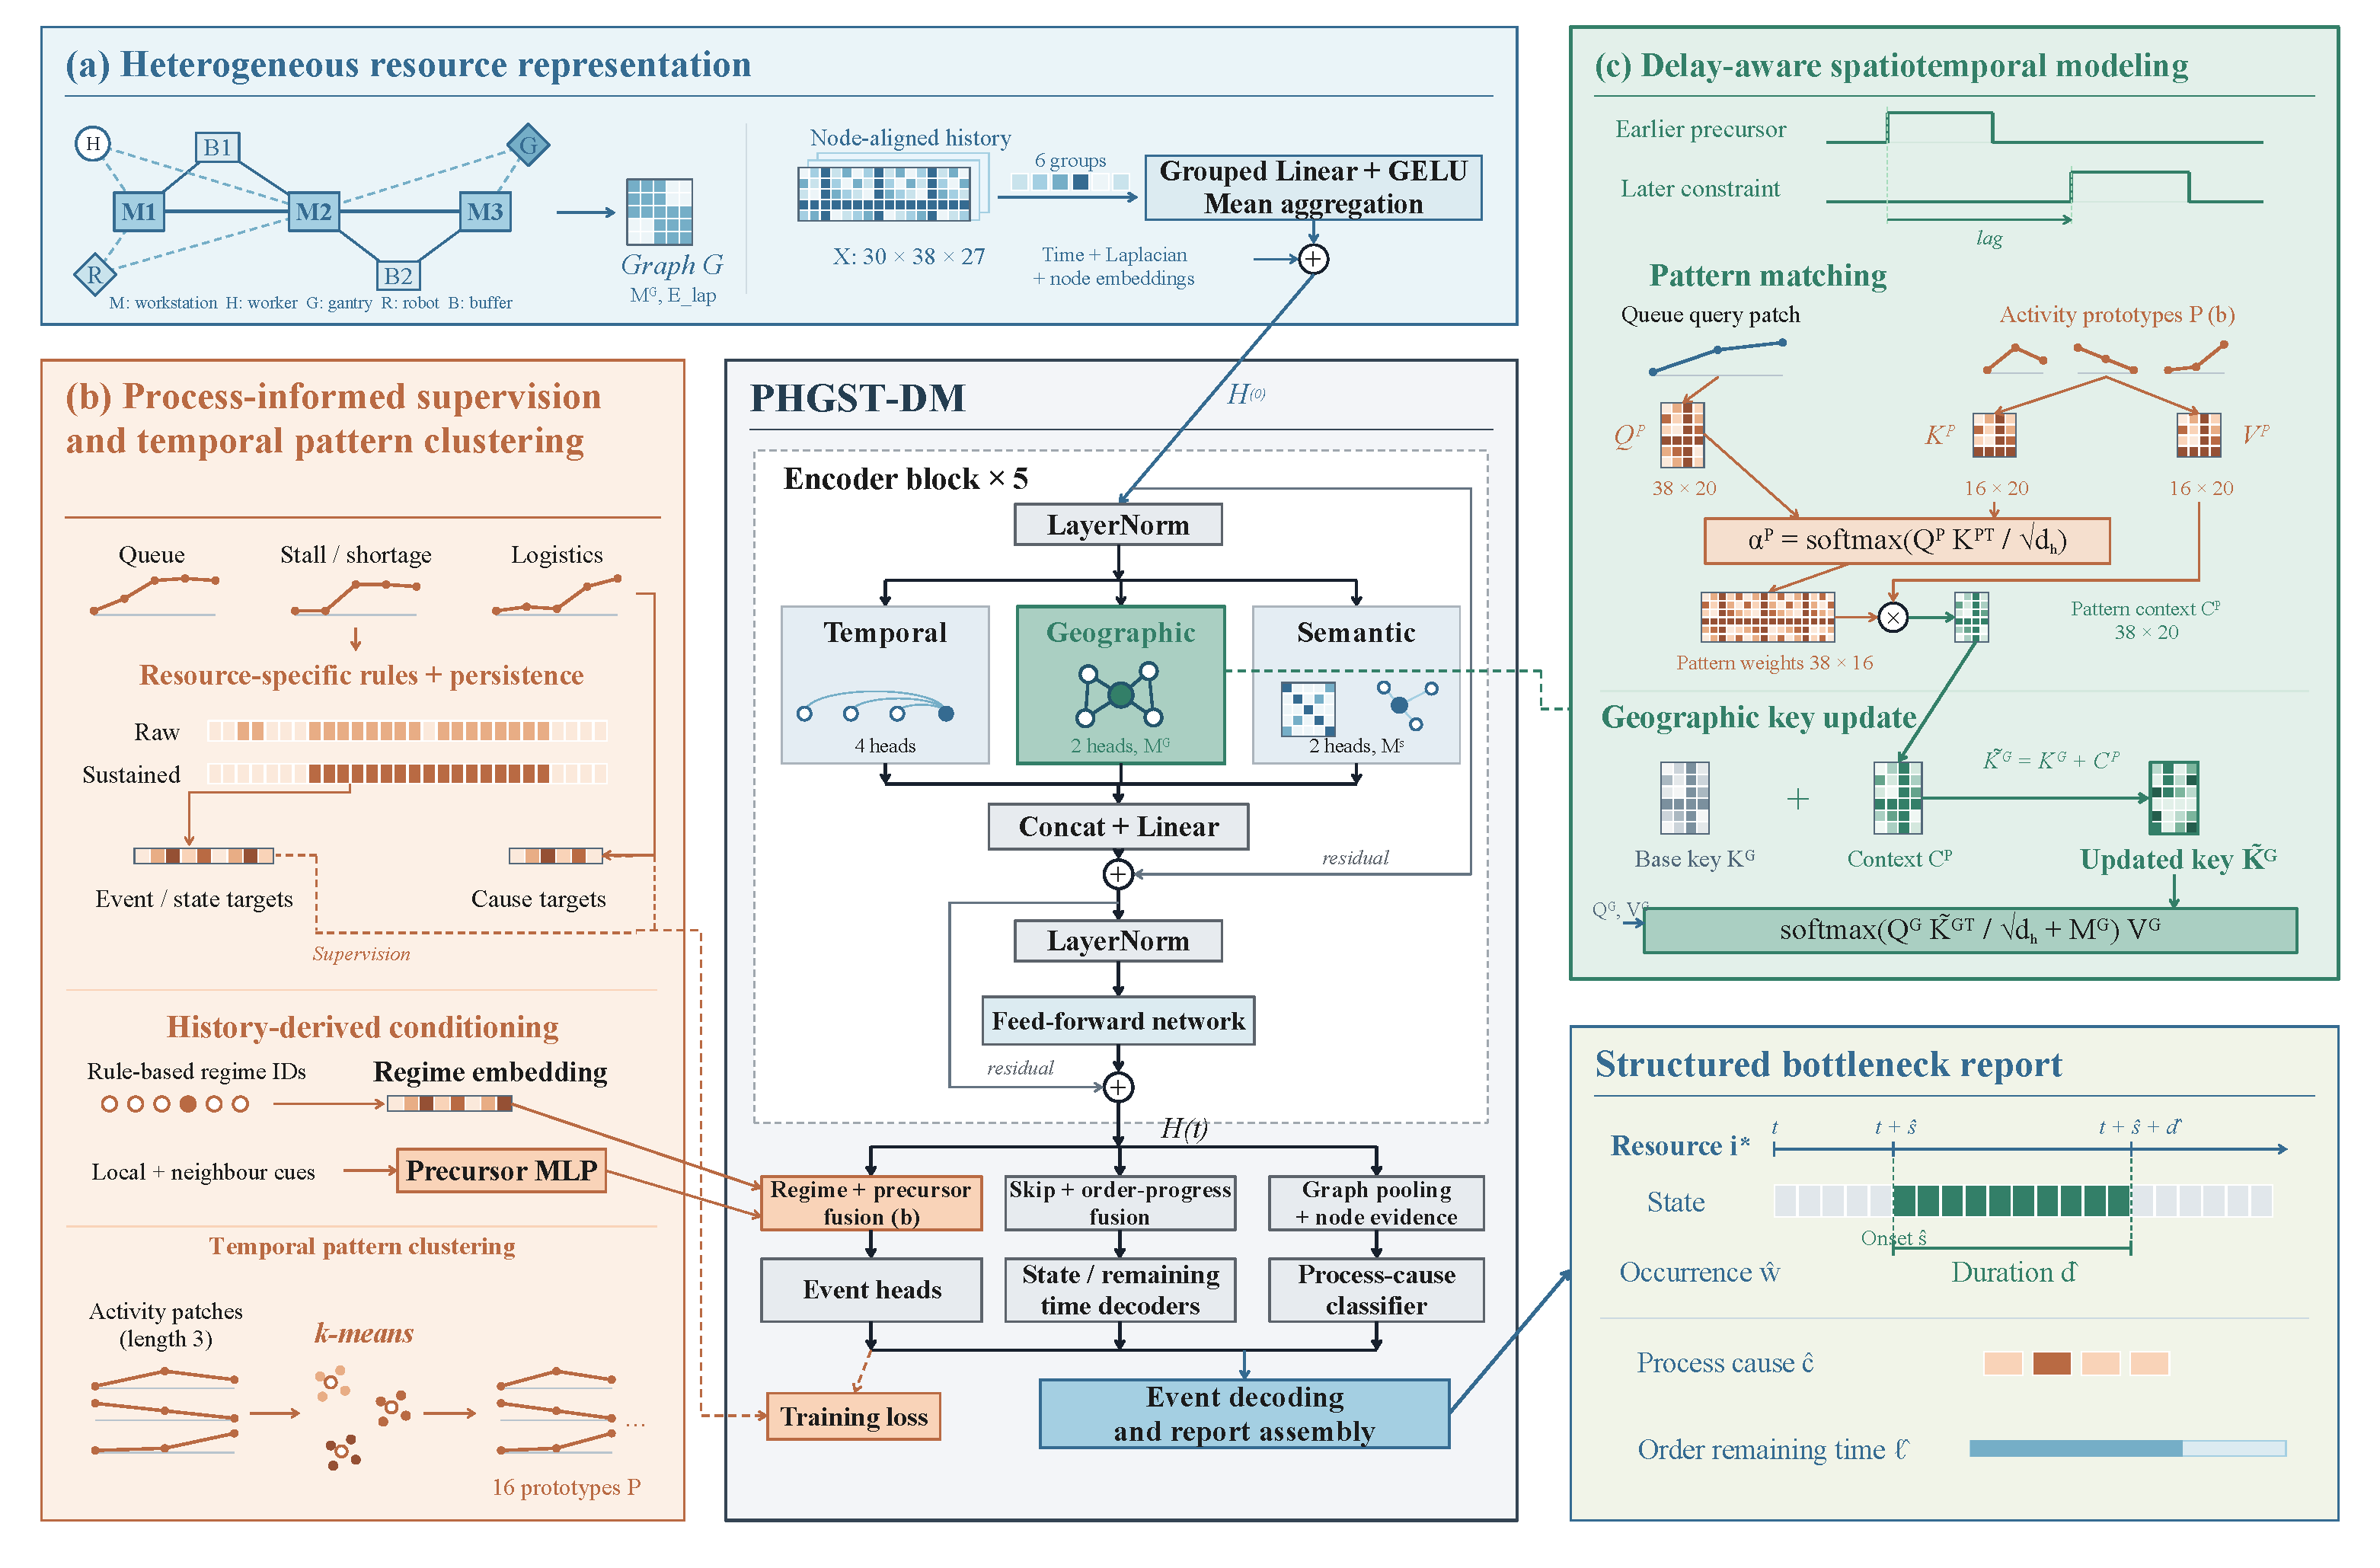
\includegraphics[width=\linewidth,height=0.62\textheight,keepaspectratio]{figures/fig_model_final.pdf}
\caption{PHGST-DM architecture and recurrent-pattern-guided geographic-attention conditioning.}
\label{fig:architecture}
\end{figure}
\FloatBarrier

\subsection{Temporal, Geographic, and Semantic Attention}\label{temporal-geographic-and-semantic-attention}

PHGST-DM uses temporal, geographic, and semantic branches in each encoder block, following the general spatiotemporal-attention design of PDFormer~\cite{jiang2023pdformer} but applying it to heterogeneous manufacturing states and relations. For branch \(b\in\{T,G,S\}\), the scaled dot-product operation is

\[
\operatorname{Attn}_b(Q_b,K_b,V_b;M_b)=
\operatorname{softmax}\!\left(\frac{Q_bK_b^{\top}}{\sqrt{d_h}}+M_b\right)V_b,
\]

where \(d_h\) is the per-head query/key dimension. The temporal branch learns dependencies within each resource's historical windows. Geographic attention uses \(M^G\) and the factory's structural neighbourhood; semantic attention uses \(M^S\) and training-history similarity. Their outputs are concatenated and projected, then processed by pre-normalized residual and feed-forward layers.

Five encoder blocks are used, each with hidden dimension \(80\). The temporal, geographic, and semantic branches contain \textbf{4, 2, and 2 heads}, respectively. A further operating-pattern context \(C^P\) conditions the geographic branch; it is defined next.

\subsection{Training-only Temporal Pattern Clustering}\label{training-only-temporal-pattern-clustering}

To summarize recurrent temporal behaviour, the model constructs a fixed prototype bank using K-means on \textbf{three-window activity-ratio patches from training histories}. The bank contains \(K=16\) prototypes, each of length \(S=3\) windows. Training-fitted feature scaling is used, the clustering initialization seed is \(0\), and the specified procedure performs ten iterations. For a patch \(p\), assignment to prototype \(k\) minimizes squared Euclidean distance:

\[
a(p)=\arg\min_{k}\lVert p-k_k^P\rVert_2^2,
\qquad
k_k^P=\frac{1}{|\mathcal{P}_k|}\sum_{p\in\mathcal{P}_k}p.
\]

The resulting pattern bank \(K^P=\{k_1^P,\dots,k_{16}^P\}\) is kept fixed during downstream model training and evaluation. These are \textbf{recurrent operating-pattern prototypes}, not labels for bottleneck presence or process causes.

Algorithm~\ref{alg:pattern-bank} specifies initialization, assignment, and centre updates. Its patch slice \(u:u+S-1\) includes both endpoints and therefore contains exactly \(S=3\) windows. Centres with no assigned patches remain unchanged, as only nonempty assignment sets are updated.

\begin{algorithm}[p]
\singlespacing
\footnotesize
\SetAlFnt{\footnotesize}
\SetAlCapFnt{\small}
\SetAlCapNameFnt{\small\bfseries}
\SetInd{0.5em}{0.8em}
\caption{Training-only temporal pattern clustering.}
\label{alg:pattern-bank}
\KwIn{scaled training histories $X^{\mathrm{tr}}$; activity channel $c_{\mathrm{act}}$; patch length $S{=}3$; centres $K{=}16$; iterations $J{=}10$; seed $0$}
\KwOut{pattern bank $K^P=\{k^P_1,\ldots,k^P_K\}$}
$\mathcal{P}\leftarrow\varnothing$\;
\ForEach{training history $X_b\in X^{\mathrm{tr}}$}{
  \ForEach{resource $n$ and valid start $u$}{
append $X_{b,u:u+S-1,n,c_{\mathrm{act}}}$ to $\mathcal{P}$\;
  }
}
initialize $K^P$ with $K$ distinct patches sampled from $\mathcal{P}$ using seed $0$\;
\For{$j=1,\ldots,J$}{
assign each $p\in\mathcal{P}$ to $a(p)=\arg\min_k\lVert p-k^P_k\rVert_2^2$\;
  \ForEach{centre $k$ with a nonempty assignment set $\mathcal{P}_k$}{
$k^P_k\leftarrow |\mathcal{P}_k|^{-1}\sum_{p\in\mathcal{P}_k}p$\;
  }
}
\Return $K^P$ reshaped to $K\times S\times1$\;
\end{algorithm}
\FloatBarrier

\subsection{Pattern-conditioned Cross-resource Interaction}\label{pattern-conditioned-cross-resource-interaction}

At prediction time, the query \(P_{t,n}\) is a \textbf{three-window queue-length patch} from the observed history, whereas the keys and values originate from the fixed \textbf{activity-ratio} prototype bank. The pattern context is

\[
C^P_{t,n}=\operatorname{softmax}\!\left(
\frac{f_Q^P(P_{t,n})\,f_K^P(K^P)^{\top}}{\sqrt{d_h}}
\right)f_V^P(K^P).
\]

The projections \(f_Q^P\), \(f_K^P\), and \(f_V^P\) are learned, but the prototype centres themselves stay fixed. The context \(C^P\) is added to the \textbf{geographic attention keys}, conditioning graph-based resource interaction on recent queue evolution matched to recurrent activity patterns. At block \(l\) the three streams may therefore be written as

\[
\begin{aligned}
H_T^{(l)}&=\operatorname{Attn}_T(H^{(l-1)}),\\
H_G^{(l)}&=\operatorname{Attn}_G(H^{(l-1)},M^G,C^P),\\
H_S^{(l)}&=\operatorname{Attn}_S(H^{(l-1)},M^S).
\end{aligned}
\]

The mechanism matches historical patches directly, \textbf{without Fourier transformation} and \textbf{without a supervised physical propagation-delay target}. It can exploit lagged predictive associations across resources, but attention maps alone are not causal explanations of how disturbances physically travel through the factory.

\section{Multi-task Bottleneck Prediction and Optimization}\label{multi-task-bottleneck-prediction-and-optimization}

\subsection{Event, Occupancy, and Explanatory Heads}\label{event-occupancy-and-explanatory-heads}

The final encoder representation is combined with deterministic regime context and local/neighbourhood precursor evidence to obtain a supervised-resource event representation \(z_{t,n}\). The model separates the prediction of an existing event's \textbf{continuation} from the \textbf{onset} of a new event:

\[
p^{\mathrm{cont}}_{t,n}=\sigma\!\left(f_{\mathrm{cont}}(z_{t,n})\right),\qquad
p^{\mathrm{onset}}_{t,n}=\sigma\!\left(f_{\mathrm{onset}}(z_{t,n})\right).
\]

The history-only state \(h_{t-1,n}\) selects the appropriate occurrence head during decoding. Additional heads produce an onset-offset distribution, predicted future duration, and prefix length:

\[
\begin{aligned}
\pi^s_{t,n}&=\operatorname{softmax}(f_s(z_{t,n})),\\
\hat d_{t,n}&=\operatorname{softplus}(f_d(z_{t,n})),\\
\hat p_{t,n}&=\operatorname{softplus}(f_p(z_{t,n})).
\end{aligned}
\]

The prefix length describes uninterrupted occupancy from the first future window and helps distinguish continued constraint from near-immediate recovery. A dense decoder predicts \(\hat O_t\in[0,1]^{H_{\mathrm{label}}\times N}\), providing future-window occupancy supervision in addition to event-level estimates.

Process-cause and remaining-order-time outputs are defined at graph level. Final node representations are pooled through a mean operation and a maximum gated-node score, then combined with order-progress information:

\[
u_t=\operatorname{AuxPool}(H_t^{(L)},\text{order state}),\qquad
\hat c_t=f_c(u_t),\quad\hat\ell_t=f_\ell(u_t).
\]

The cause head estimates rule-defined observed process conditions (Section~\ref{process-cause-and-remaining-order-time-targets}); it is not a ground-truth physical root-cause diagnosis. The remaining-time head estimates order-level progress rather than a second station-event duration.

\subsection{Joint Training Objective}\label{joint-training-objective}

The training objective combines event occurrence, onset, temporal regression, occupancy, auxiliary outputs, and representation regularization:

\[
\begin{aligned}
\mathcal{L}={}&\lambda_w\mathcal{L}_{\mathrm{will}}+\lambda_{on}\mathcal{L}_{\mathrm{onset}}+
\lambda_s\mathcal{L}_{\mathrm{start}}+\lambda_d\mathcal{L}_{\mathrm{dur}}\\
&+\lambda_p\mathcal{L}_{\mathrm{prefix}}+\lambda_o\mathcal{L}_{\mathrm{occ}}+
\lambda_{\ell}\mathcal{L}_{\mathrm{remain}}+\lambda_c\mathcal{L}_{\mathrm{cause}}\\
&+\lambda_r\mathcal{L}_{\mathrm{recon}}+\lambda_q\mathcal{L}_{\mathrm{contrast}}+
\lambda_{\mathrm{tpm}}\mathcal{L}_{\mathrm{tpm}}.
\end{aligned}
\]

Occurrence prediction combines reweighted binary cross-entropy, focal modulation, hard-false-positive weighting, and an internal differentiable F1 term. The new-onset head receives separate onset supervision. A Gaussian soft target supports onset-offset prediction, while log-transformed Smooth-L1 losses are used for duration, prefix, and remaining-time regression. The occupancy objective combines type-balanced binary cross-entropy with soft Dice and soft intersection-over-union terms. Class-weighted process-cause cross-entropy is applied only where a supported cause label accompanies positive bottleneck evidence. Reconstruction and supervised contrastive losses regularize the shared representation, and an auxiliary turning-point loss is included in the final objective.

One naming distinction matters for reproducing the configuration. The active event-occurrence term \(\mathcal{L}_{\mathrm{will}}\) is \textbf{not} the same as the disabled legacy configuration switch named \texttt{will}. The offline cluster-head weight is zero, \(\lambda_{\mathrm{cluster}}=0\), so the model is not trained to classify offline cluster assignments. Key loss weights and decoding thresholds are specified in Section~\ref{sec:experimental-settings}.

\subsection{Two-stage Training and Validation-controlled Decoding}\label{two-stage-training-and-validation-controlled-decoding}

\textbf{Stage 1: joint representation and event learning.} Training initializes the model from the documented prefix-supervised checkpoint and follows the onset-limit curriculum \(5\rightarrow10\rightarrow15\) minutes. When available, the retained checkpoint from one onset-limit setting warm-starts the next. Fourfold positive-window oversampling addresses the rarity of event-bearing samples. Far-onset enhancement and weighted false-positive penalties balance warning sensitivity against false reports. The optimizer is AdamW with batch size 16, an initial learning rate of \(5\times10^{-5}\), weight decay \(0.05\), and cosine decay towards \(10^{-6}\). The shared training protocol uses at most 50 epochs per onset-limit run and early-stopping patience 40.

\textbf{Validation selection.} Candidate checkpoints and report thresholds are evaluated only on the validation episodes. Checkpoint selection uses specified precision/recall gates and station-identification F1, with a validation-only fallback when the gates cannot be met. Candidate report thresholds are drawn from the documented set from 0.45 through 0.94. Once selected, the event model and threshold are frozen before any held-out test evaluation.

\textbf{Stage 2: remaining-time specialization.} The encoder and event, occupancy, and cause heads are frozen, while a rate-augmented remaining-time head is optimized using a progress-weighted objective. This stage does not retune the event threshold and does not change the frozen event or cause outputs. The finalized study uses seed 42; its principal experiments are single-seed estimates rather than multi-seed uncertainty measurements.

\textbf{Inference and report generation.} The decoder uses the observed-prefix state \(h_{t-1,n}\) to select the continuation score for an active resource or the new-onset score otherwise. Prefix evidence may retain an ongoing event with onset offset zero. An eligible occupancy run is extracted from the predicted occupancy grid and combined with event-head estimates under the appropriate duration rules. Global and resource-type thresholds, together with the active onset limit, determine which reports are retained. Each retained report contains resource identity, onset, predicted duration, the graph-level process-cause output, and remaining order time.

For strict evaluation, a matched report must identify the correct resource and satisfy an onset-offset tolerance of three one-minute windows:

\[
|\hat s_{t,n}-s_{t,n}|\leq\epsilon_s,\qquad \epsilon_s=3\ \mathrm{min}.
\]

This onset-qualified event metric is distinct from the internal station-identification score used during validation selection. Chapter~\ref{ch:experiments} details the evaluation results. Throughout the pipeline, held-out episodes are not used to fit scalers, masks, prototypes, neural parameters, or reporting thresholds.

Algorithm~\ref{alg:phgst-predict} formalizes the forward pass and report decoder. The symbols \(a_n^{\mathrm{cont}}\) and \(a_n^{\mathrm{onset}}\) denote head scores; their sigmoid probabilities correspond to \(p^{\mathrm{cont}}\) and \(p^{\mathrm{onset}}\). The residual updates abbreviate the pre-normalized encoder described in Section~\ref{temporal-geographic-and-semantic-attention}. The observed-prefix continuation cutoff is 1.5 windows, and occupancy runs use cutoff 0.45. Upcoming reports obey the onset limit and minimum-duration rule; ongoing duration describes the future remainder. Section~\ref{sec:experimental-settings} supplies the global and resource-type thresholds and full loss settings.

\begin{algorithm}[p]
\singlespacing
\footnotesize
\SetAlFnt{\footnotesize}
\SetAlCapFnt{\small}
\SetAlCapNameFnt{\small\bfseries}
\SetInd{0.5em}{0.8em}
\caption{PHGST-DM prediction with delay-aware spatiotemporal modelling.}
\label{alg:phgst-predict}
\KwIn{history $X_t$ and history-only state $h_{t-1}$; $A,M^{G},M^{S}$; pattern bank $K^{P}$; regime state $r_{t-1}$; parameters $(\theta,\psi)$; threshold $\tau$; onset limit $H_{\mathrm{start}}$}
\KwOut{station reports $\widehat{\mathcal{R}}_t$; occupancy $\hat O_t$; cause $\hat c_t$; remaining time $\hat\ell_t$}
\BlankLine
\textbf{Phase 1: heterogeneous state representation}\;
\ForEach{group $q$}{
$e^{(q)}\leftarrow\mathrm{GELU}(W_q x^{(q)}+b_q)$\;
}
$H^{(0)}\leftarrow\mathrm{mean}_{q}e^{(q)}+E_{\mathrm{time}}+E_{\mathrm{lap}}+E_{\mathrm{node}}$\;
construct history-only queue patches $P$ of length $3$ and project the fixed activity-pattern centres $K^{P}$\;
\BlankLine
\textbf{Phase 2: delay-aware spatiotemporal modelling}\;
\For{$l\leftarrow 1$ \KwTo $5$}{
$H_T\leftarrow\mathrm{Attn}_{T}(H^{(l-1)})$\;
$C^{P}\leftarrow\mathrm{softmax}(f_Q^{P}(P)f_K^{P}(K^{P})^{\top}/\sqrt{d_h})f_V^{P}(K^{P})$ \tcp*{queue query vs.\ activity prototypes}
$H_G\leftarrow\mathrm{Attn}_{G}(H^{(l-1)},M^{G};\,\text{geographic keys}+C^{P})$ \tcp*{delay-aware geographic mixing}
$H_S\leftarrow\mathrm{Attn}_{S}(H^{(l-1)},M^{S})$\;
$\widetilde H^{(l)}\leftarrow H^{(l-1)}+\mathrm{Proj}[H_T;H_G;H_S]$\;
$H^{(l)}\leftarrow\widetilde H^{(l)}+\mathrm{FFN}(\widetilde H^{(l)})$\;
}
\BlankLine
\textbf{Phase 3: station-level and graph-level prediction heads}\;
$z_n\leftarrow H^{(5)}_{t-1,n}+E_{\mathrm{regime}}(r_{t-1,n})$ for the station-event branch\;
fuse local queue/stall and neighbourhood precursor evidence into $z_n$\;
\ForEach{$n\in\mathcal{S}$}{
$(a^{\mathrm{cont}}_n,a^{\mathrm{onset}}_n)\leftarrow(f_{\mathrm{cont}}(z_n),f_{\mathrm{onset}}(z_n))$ \tcp*{continuation vs.\ new-onset scores}
$(\pi^{s}_n,\hat d_n,\hat p_n)\leftarrow(\mathrm{softmax}(f_s(z_n)),\mathrm{softplus}(f_d(z_n)),\mathrm{softplus}(f_p(z_n)))$\;
}
$\hat O_t\leftarrow\sigma(f_O(H^{(5)}))$; pool nodes and order progress into $u_t$; set $(\hat c_t,\hat\ell_t)\leftarrow(f_c(u_t),f_{\psi}(u_t))$\;
\BlankLine
\textbf{Phase 4: event-consistent operational decoding}\;
$\widehat{\mathcal{R}}_t\leftarrow\varnothing$\;
\ForEach{$n\in\mathcal{S}$}{
select $a_n\leftarrow a^{\mathrm{cont}}_n$ if $h_{t-1,n}=1$, and $a_n\leftarrow a^{\mathrm{onset}}_n$ otherwise\;
  \If{$h_{t-1,n}=1$ and $\hat p_n$ satisfies the continuation rule}{
lift $a_n$ with prefix evidence and set $\hat s_n\leftarrow0$\;
  }
recover the longest eligible run $(\hat s^{O}_n,\hat d^{O}_n)$ from $\hat O_{t,:,n}$\;
merge the run and event-head estimates subject to the ongoing/upcoming duration rule\;
apply the global threshold $\tau$, the resource-type threshold, and the onset limit $H_{\mathrm{start}}$\;
  \If{station $n$ is retained}{
append $(n,\hat s_n,\hat d_n,\hat c_t,\hat\ell_t)$ to $\widehat{\mathcal{R}}_t$\;
  }
}
\Return $\widehat{\mathcal{R}}_t,\hat O_t,\hat c_t,\hat\ell_t$\;
\end{algorithm}
\FloatBarrier

\section{Production-sensitivity Validation Protocol}\label{production-sensitivity-validation-protocol}

Predictive agreement with process-informed labels alone does not establish that the labels rank resources according to their influence on production completion. To examine this question, the study separately performs a counterfactual \textbf{production-sensitivity replay}. This procedure is independent of PHGST-DM training and inference.

At saved factory state \(t\), each of seven workstation candidates is evaluated through a separate service-bundle acceleration. Workstation processing and associated worker service durations are multiplied by \(0.8\), corresponding to a \(1.25\times\) service rate, for 1,200 simulation steps. Baseline and intervention branches start from the same saved factory and random-number states and run until order completion. For workstation \(i\), sensitivity is the reduction in remaining completion time:

\[
S_i(t)=M_{\mathrm{base}}(t)-M_{i,0.8}(t),
\]

where \(M_{\mathrm{base}}(t)\) and \(M_{i,0.8}(t)\) are measured from the same origin. Positive \(S_i(t)\) means that the specified temporary acceleration shortens the order's completion time.

Label-based rankings are formed using the maximum evidence in the last three fully observed windows before \(t\). Their alignment with counterfactual sensitivity is evaluated using \textbf{NDCG@3}, \textbf{Positive Recall@\(k\)}, \textbf{Weighted Recall@3}, and \textbf{Coverage@3} under a 90\%-of-maximum sensitivity criterion. NDCG@3 evaluates ranked relevance; Positive Recall@\(k\) covers the oracle's highest positive-sensitivity candidates; Weighted Recall@3 captures the proportion of total positive sensitivity ranked among the first three; and Coverage@3 assesses whether near-maximally sensitive resources appear among the first three candidates.

The protocol tests whether the operational labels agree with a specific, fixed acceleration intervention in the simulated factory. It does \textbf{not} demonstrate a general causal explanation of bottleneck events, the effectiveness of a learned intervention policy, or throughput improvement from forecast-guided closed-loop control. Its pilot results are presented in Section~\ref{sec:supervision-analysis}, while generalization limits and future validation directions are discussed in Chapter~\ref{ch:conclusion}.

In summary, the methodology brings together multi-entity factory observations, process-informed persistent-event supervision, a weighted heterogeneous process--logistics graph, and recurrent-pattern-conditioned spatiotemporal attention. It predicts resource-level event occurrence and timing together with observable process context and order progress, while maintaining a strict boundary between retrospective supervision and information available at the forecast origin.
